\documentclass[12pt,a4paper]{article}

% Paquetes básicos
\usepackage[x11names]{xcolor}
\usepackage[utf8]{inputenc}
\usepackage{mathtools, amssymb, amsthm}
\usepackage{changepage}
\usepackage{geometry}
\usepackage[colorlinks=true]{hyperref}
\usepackage{enumitem}
\usepackage{etoolbox}
\usepackage{graphicx}
\usepackage{setspace}
\usepackage{tcolorbox}
\tcbuselibrary{skins, breakable}
\usepackage{titlesec}
\usepackage{tikz} % core TikZ
\usetikzlibrary{matrix}
\usepackage{pgfplots}
\pgfplotsset{compat=newest}
\usepgfplotslibrary{fillbetween}

% Margins
%\geometry{left=3cm,right=3cm,top=2.5cm,bottom=2.5cm}

% Custom operators
\newcommand{\card}{\operatorname{card}}
\newcommand{\muae}{\overset{\mu-a.e.}{=}}

% Implication box setup
\tcbset{Implication-number/.style={
  enhanced,
  boxsep=2pt,
  colback=white,
  frame hidden,
  sharp corners,
  left=2pt, right=2pt, top=1pt, bottom=1pt,
  underlay={
    \draw[line width=0.5pt] (frame.south west) -- ([xshift=-133mm]frame.south east); % línea horizontal
    \draw[line width=0.5pt] ([xshift=-133mm]frame.north east) -- ([xshift=-133mm]frame.south east); % línea vertical
  }
}}

\tcbset{Implication-number-ds/.style={
  enhanced,
  boxsep=2pt,
  colback=white,
  frame hidden,
  sharp corners,
  left=2pt, right=2pt, top=1pt, bottom=1pt,
  underlay={
    \draw[line width=0.5pt] ([yshift=5mm]frame.south west) -- ([xshift=-133mm, yshift=5mm]frame.south east); % línea horizontal
    \draw[line width=0.5pt] ([xshift=-133mm, yshift=-3mm]frame.north east) -- ([xshift=-133mm, yshift=5mm]frame.south east); % línea vertical
  }
}}

\tcbset{Subset-contingency/.style={
  enhanced,
  boxsep=2pt,
  colback=white,
  frame hidden,
  sharp corners,
  left=2pt, right=2pt, top=1pt, bottom=1pt,
  underlay={
    \draw[line width=0.5pt] (frame.south west) -- ([xshift=-140mm]frame.south east); % línea horizontal
    \draw[line width=0.5pt] ([xshift=-140mm]frame.north east) -- ([xshift=-140mm]frame.south east); % línea vertical
  }
}}

\tcbset{Indent-subset-contingency/.style={
  enhanced,
  boxsep=2pt,
  colback=white,
  frame hidden,
  sharp corners,
  left=2pt, right=2pt, top=1pt, bottom=1pt,
  underlay={
    \draw[line width=0.5pt] (frame.south west) -- ([xshift=-140mm+0.07\textwidth]frame.south east); % línea horizontal
    \draw[line width=0.5pt] ([xshift=-140mm+0.07\textwidth]frame.north east) -- ([xshift=-140mm+0.07\textwidth]frame.south east); % línea vertical
  }
}}

% Useful commands
\renewcommand{\contentsname}{Contenidos}

\newcommand{\R}{\mathbb{R}}
\newcommand{\N}{\mathbb{N}}
\newcommand{\Z}{\mathbb{Z}}
\newcommand{\Q}{\mathbb{Q}}
\newcommand{\C}{\mathbb{C}}

\newcommand{\smallcup}{\mathop{\cup}\limits}
\newcommand{\smallcap}{\mathop{\cap}\limits}
\newcommand{\smallsum}{\mathop{\sum}\limits}
\newcommand{\smallprod}{\mathop{\prod}\limits}

\newcommand{\linf}[1]{\displaystyle{\mathop{\underline{\lim}}_{#1}}}
\newcommand{\mlim}[1]{\displaystyle{\lim_{#1}}}

%Integral de Lebesgue con patas
\newcommand{\lbint}{\mathop{\int_{\!\!\!\!\!|\!}^{\!|\!}}}

%Espacios \mathcal{L}_p
\newcommand{\elep}[2]{\mathcal{L}_{#1}(#2)}

% ----- Custom counters and counter commands -----
% Custom counter hierarchy
\newcounter{unit}[section]
\newcounter{chapter}[unit]
\makeatletter
\@addtoreset{subsubsection}{chapter}
\makeatother

\renewcommand{\theunit}{\arabic{unit}}
\renewcommand{\thechapter}{\arabic{chapter}}
\renewcommand{\thesubsubsection}{\theunit.\thechapter.\arabic{subsubsection}}

% Custom content hierarchy behavior
\newcommand{\chapter}[1]{
    \refstepcounter{chapter}
    \subsection*{\Large{\S \thechapter. #1}}
    \addcontentsline{toc}{subsection}{\thechapter. #1}
}
\newcommand{\unit}[1]{
    \refstepcounter{unit}
    \section*{\Huge{\Roman{unit} #1}}
    \addcontentsline{toc}{section}{\Roman{unit} #1}
}

\newcommand{\result}[1]{%
  \subsubsection{#1}%
  \label{result:\thesubsubsection}
}
  
\titleformat{\subsubsection}
    {\normalfont\large\bfseries} % mismo tamaño que \subsection
    {\thesubsubsection}{1em}{}
  
%---- Custom proof commands-----
\newcommand{\dem}{
    \noindent \underline{\textbf{Demostración:}}
}
\newcommand{\nota}{
    \noindent \underline{\textbf{Nota:}}
}
% ----------------------------------------
\hbadness=10000
\vbadness=10000
\hfuzz=100pt
\vfuzz=100pt
% ---------------------------------------
\title{Análisis Matemático III}
\author{Javier Ortín Rodenas}
\date{Curso 2025-2026}


\begin{document}

\maketitle
\newpage
\hypersetup{linkcolor=black}
\tableofcontents
\hypersetup{linkcolor=Ivory4}
\newpage
\setcounter{unit}{3}
\unit{Series de Fourier}
\hspace{3mm} Recordamos que ${L}_2(X,K) \equiv \frac{\mathcal{L}_2(X,K)}{\sim}$ es un espacio de Hilbert; donde $X$ es un $K-$espacio vectorial, y $f \sim g \iff f \muae g$. El producto interior y su norma asociada se definen como:
\begin{align*}
    \langle f,g\rangle = \int_X \bar{f} \cdot g && ||f||_2 = \sqrt{\langle f,f\rangle}
\end{align*}
Nótese que cuando trabajamos con $\C$ como cuerpo el producto interno tiene linealidad directa en una componente, mientras que tiene linealidad por el conjugado en la otra. Asimismo, el producto interno da lugar a escalares del propio cuerpo sobre el que se define, luego podría dar lugar a valores complejos. Además, el producto interno no conmuta (en general) en $\C$.

\vspace{4mm}
La idea de esta unidad es ``aproximar'' una función $f \in L_2(X,K)$ como ``suma'' de funciones más elementales. En particular, a partir de ahora, consideraremos $X = I = [0,2\pi]$, con $K = \R$ ó $\C$. Además, extenderemos las funciones en este conjunto con periodicidad $2\pi$ en $\R$.

\vspace{6mm} 
\chapter{Primeros conceptos}
\result{Definición de sistema ortonormal}
\hspace{3mm} Dado un espacio de Hilbert $V$, un sistema ortonormal en $V$ es un conjunto $\{\varphi_n\}_{n\in\N} \subseteq V$ que verifica:
$$\langle\varphi_n, \varphi_m\rangle = \delta_{n,m} = \begin{cases}
  1 & \text{ si } n = m \\
  0 & \text{ si } n \neq m
\end{cases}$$

\vspace{6mm}
\result{Ejemplos de sistemas ortonormales}
\begin{enumerate}[label=\roman*)]
    \item $K = \R$, $V = L_2([0,2\pi], \R)$. Consideramos el siguiente sistema:
    \begin{align*}
        \varphi_0(t) =  \frac{1}{\sqrt{2\pi}} &&
        \varphi_{2n-1}(t) = \frac{\cos (nt)}{\sqrt{\pi}} &&
        \varphi_{2n}(t) = \frac{\sin (nt)}{\sqrt{\pi}}
    \end{align*}
    Veamos que es ortonormal:
    \begin{flalign*}
        \int_0^{2\pi} \varphi_0^2(t) \,dt = \int_{0}^{2\pi}\frac{1}{2\pi}\,dt = 1&&
    \end{flalign*}
    \begin{flalign*}
        \int_0^{2\pi} \varphi_{2n+1}^2(t) \,dt &= \int_{0}^{2\pi}\frac{\cos^2(nt)}{\pi}\,dt \overset{u = nt}{=} \frac{1}{n\pi}\int_{0}^{2n\pi}\frac{1+\cos(2u)}{2}du \overset{v=2u}{=} &&\\
        &=\frac{1}{4n\pi} \int_{0}^{4n\pi} 1+ cos(v) = \frac{4n\pi}{4n\pi} + 0= 1
    \end{flalign*}
    \begin{flalign*}
        \int_0^{2\pi} \varphi_{2n}^2(t) \,dt &= \int_{0}^{2\pi}\frac{\sin^2(nt)}{\pi}\,dt \overset{u = nt}{=} \frac{1}{n\pi}\int_{0}^{2n\pi}\frac{1-\cos(2u)}{2}du \overset{v=2u}{=}&&\\
        &=\frac{1}{4n\pi} \int_{0}^{4n\pi} 1-(v) = \frac{4n\pi}{4n\pi} + 0 = 1
    \end{flalign*}
    Por ser funciones con periodo $2\pi$, para $n \in \N$ cualquiera, se cumple:
    $$ \int_{0}^{2\pi}\varphi_{2n+1}(t)\,dt=\int_{0}^{2\pi}\varphi_{2n}(t)\,dt= \int_{0}^{2\pi}\varphi_{2n+1}(t)\cdot\varphi_{2n}(t)\,dt= 0$$
    Hemos demostrado que el sistema es ortonormal.
    
    \vspace{8mm}
    \item Para $K = \C$, $V = L_2([0,2\pi], \C)$, el siguiente sistema es ortonormal:
    $$ \left\{\varphi_n(t) = \frac{e^{i\cdot n\cdot t}}{\sqrt{\pi}}\right\}_{n\in\N}$$
\end{enumerate}

\vspace{6mm}  
\result{Teorema de óptima aproximación}
\hspace{3mm} Sea $V$ un $K$-espacio pre-Hilbert. Sea $\{\varphi_0, \ldots,\varphi_n\} \subseteq V$ un sistema ortonormal finito en $V$. Sea $f \in V$. Si $W$ es la clausura $K\langle \varphi_0,\ldots,\varphi_n\rangle$. Entonces, el elemento de $W$ que mejor aproxima $f$ (en cuanto a minimizar la norma de su diferencia) es
$$ s_n = \sum_{k=0}^n \underbracket{\langle f, \varphi_k\rangle>}_{c_k}\varphi_k$$
Es decir, dado $t_n = \smallsum_{k=0}^n b_k \cdot \varphi_k \in W$ cualquiera (formado a partir de escalares cualesquiera), se cumple $||f-s_n|| \leq ||f-t_n||$.

\newpage\dem 
\vspace{2mm} \newline \indent Al ser un espacio Pre-Hilbert por hipótesis, tenemos que :
\begin{flalign*}
    ||f &-t_n||^2 = \langle f-t_n, f-t_n\rangle = \langle f,f\rangle - \langle f, t_n\rangle - \langle t_n, f\rangle + \langle t_n, t_n\rangle =&&\\[2ex]
    &= ||f||^2 - \left\langle f, \sum_{k=0}^{n}b_k \varphi_k\right\rangle - \left\langle \sum_{k=0}^n b_k \varphi_k, f\right\rangle + \left\langle \sum_{k=0}^n b_k \varphi_k, \sum_{k=0}^n b_k \varphi_k\right\rangle = \substack{\text{linealidad}\\[1ex] \text{ortonormalidad}} \\[2ex]
    &= ||f||^2 - \sum_{k=0}^n{b_k} \langle f,  \varphi_k\rangle
    - \sum_{k=0}^n\bar{b}_k \langle f,  \varphi_k\rangle + \sum_{k=0}^{n} \bar{b}_k \cdot b_k = \text{definición de }c_k \\
    &= ||f||^2 + \sum_{k=0}^n \Big[-b_k c_k - \bar{b}_k c_k + |b_k|^2\Big] = (*)
\end{flalign*}
Comparamos ahora con la siguiente expresión:
$$|b_k - c_k|^2 = (b_k - c_k)(\bar{b}_k - \bar{c}_k) = b_k \bar{b_k} - b_k \bar{c}_k - \bar{b}_k c_k + c_k \bar{c}_k = |b_k|^2 + |c_k|^2 - b_k \bar{c}_k - \bar{b}_k c_k$$
\vspace{2mm}
Sustituyendo en la igualdad anterior,
$$(*) = ||f||^2 + \sum_{k=0}^{n}\Big[ |b_k-c_k|^2 - |c_k|^2 \Big]$$
En particular, para $b_k = c_k$ tenemos $||f-s_n||^2 \leq ||f-t_n||^2$.

\vspace{4mm}
Motivados por este resultado, buscamos aproximar $f$ por una ``combinación lineal infinita'' de funciones de un sistema ortonormal.

\vspace{6mm}
\result{Definición de coeficientes de Fourier}
\hspace{3mm} Dada una función $f \in L_2([0,2\pi])$, y un sistema ortonormal $\{\varphi_n\}_{n\in\N}$. Se denomina ``coeficiente $n$-ésimo de Fourier de $f$ respecto de $\{\varphi_n\}_{n\in\N}$'' al escalar:
$$ c_n := \langle f, \varphi_n\rangle = \int_{0}^{2\pi} \bar{f}(t)\cdot \varphi_n(t) \,dt$$
Definimos la suma parcial $n$-ésima de Fourier de $f$ respecto de $\{\varphi_n\}_{n\in\N}$ como:
$$s_n(x) = \sum_{k=0}^n c_k \cdot \varphi_k(x)$$
Análogamente, la serie de Fourier de $f$ respecto de $\{\varphi_n\}_{n\in\N}$ viene dada po:
$$s(x) = \sum_{k=0}^\infty c_k \cdot \varphi_k(x)$$

\vspace{6mm}
\result{Unicidad de las Series de Fourier}
\hspace{3mm} Sea $f \in L_2(I,K)$. Sea $\{\varphi_n\}_{n\in\N}$ un sistema ortonormal. La serie de Fourier de $f$ respecto de $\{\varphi_n\}_{n\in\N}$ está bien definida, pues existe un único elemento $s \in L_2(I,K)$ que verifica:
$$||s-s_n|| \xrightarrow{n\to\infty}0$$

\vspace{4mm} \dem
\vspace{2mm} \newline \indent Sean $p,q$ in $\N$ cualesquiera. Supongamos sin pérdida de generalidad que $q > p$. Entonces,
\begin{flalign*}
  ||s_p -& s_q||^2 = \left|\left| \sum_{k=p+1}^q s_k \right|\right|^2 = \left\langle\sum_{k=p+1}^{q}\langle f, \varphi_k\rangle \varphi_k,\sum_{k=p+1}^{q}\langle f, \varphi_k\rangle \varphi_k\right\rangle \overset{\text{ortonormalidad}}{=} &&\\
  &= \sum_{k=p+1}^q \left|\langle f, \varphi_k\rangle\right|^2 = |a_p - a_q|^2 \hspace{4ex} \text{ donde } a_n = \sum_{k=0}^{n} |\langle f, \varphi_k\rangle|^2
\end{flalign*}
\vspace{2mm}
Por el \hyperref[result:4.1.3]{Teorema de óptima aproximación}, para $n \in \N$ cualquiera tenemos que:
$$||f-s_n||^2 = ||f||^2 - \underbracket{\sum_{k=0}^n |\langle f, \varphi_k\rangle|^2}_{a_n} = ||f||^2 - a_n$$
Esto implica que $||f||^2 \geq a_n$. Así, tomando límites en $n$ tenemos que:
$$a := \sum_{k=0}^\infty|\langle f, \varphi_k\rangle|^2 \leq ||f||^2$$
Esta es la conocida como \textbf{Desigualdad de Bessel}.

\vspace{2mm}
Por tanto, tenemos que $(a_n)_n$ es de Cauchy, luego $(s_n)_n$ ha de serlo también. Al estar además en un espacio de Banach, podemos asegurarnos de que $(s_n)_n$ es convergente a $s$.

\vspace{4mm}
\nota \vspace{2mm} \newline \indent
Este resultado garantiza la convergencia en norma de las sumas parciales de Fourier a su límite. No tiene por qué darse $f(x) = s(x)$. Cabe preguntarse si esto es a su vez equivalente a $||f-s_n|| \xrightarrow{n\to\infty}0$. Pasaremos a estudiar escenarios donde puede ocurrir.

\vspace{6mm}
\result{Identidad de Parseval}
\hspace{3mm} Sea $f \in L_2(I,K)$. Sea $\{\varphi_n\}_{n\in\N} \subseteq L_2(I,K)$ un sistema ortonormal. Sea $c_n := \langle f, \varphi_n\rangle$ para cada $n\in\N$. Entonces,
$$||f-s_n|| \xrightarrow{n\to\infty} 0 \iff \sum_{n=0}^\infty |c_n|^2 = ||f||^2$$

\vspace{4mm} \dem
\vspace{2mm} \newline \indent Por el \hyperref[result:4.1.3]{Teorema de óptima aproximación}, sabemos que:
$$||f-s_n||^2 = ||f||^2 - \sum_{k=0}^{n} |c_k|^2 \hspace{2mm}  \forall \hspace{1mm} n \in \N$$
Despejamos y tomamos límites:
$$\lim_n ||f-s_n||^2 = 0 \iff \sum_{k=0}^{\infty} |c_k|^2 = ||f||^2$$

\vspace{6mm}
\result{Definición de sistema ortonormal completo}
\hspace{3mm} Sea $H$ un espacio de Hilbert. Sea $\{\varphi_n\}_{n\in\N}$ un sistema ortonormal. Se dice ``completo'' si satisface la Identidad de Parseval para cualquier $f \in H$. Es decir,
$$\sum_{k=0}^{\infty}\langle f, \varphi_k\rangle = ||f||^2 \hspace{3mm} \forall \hspace{1mm} f \in H$$

\newpage
\nota
\vspace{2mm} \newline \indent Por la \hyperref[result:4.1.5]{Desigualdad de Bessel}, sabemos que $\smallsum_{k=0}^{\infty}|c_k|^2 \leq ||f||^2$. Exigir la igualdad equivale a decir que la norma se resume completamente por el sistema ortonormal: el sistema puede aportar información sobre todo el espacio $H$. Por tanto, toda componente de $f$ queda recogida por cierto $\varphi_n$, luego $f \neq 0$ implica que no es ortogonal a todo el sistema.

\vspace{6mm}
\result{Ejemplo de sistema ortonormal completo}
\hspace{3mm} En $L_2(I,K)$, el siguiente sistema ortonormal es completo:
$$\left\{\frac{1}{\sqrt{2\pi}}, \frac{\cos(t)}{\sqrt{\pi}}, \frac{\sin(t)}{\sqrt{\pi}}, \frac{\cos(2t)}{\sqrt{\pi}}, \frac{\sin(2t)}{\sqrt{\pi}},\ldots\right\} $$
La demostración es demasiado larga, luego no se verá.

\vspace{4mm} Este es el sistema ortonormal más utilizado, y la serie de Fourier de una función $f$ respecto de él, se denomina simplemente ``serie de Fourier de $f$''. Viene representada por:
$$f(t) \sim \frac{a_0}{2} + \sum_{n=1}^{\infty}\Big[a_n\cos(nt) + b_n\sin(nt)\Big]$$
Donde ``$\sim$'' significa convergencia en media cuadrática. Podemos obtener los coeficientes $a_n,b_n$ por identificación al aplicar la ortonormalidad. Por definición, la suma parcial $k$-ésima de Fourier de $f$ viene dada por:
$$s_k(t) = \sum_{n=0}^{k} \langle f, \varphi_n\rangle \hspace{1mm} \varphi_n(t) = \frac{c_0}{\sqrt{2\pi}} + \sum_{n=1}^{k}\left[c_{2n-1}\frac{\cos(nt)}{\sqrt{\pi}}+c_{2n}\frac{\sin(nt)}{\sqrt{\pi}}\right]$$
\vspace{2mm} De este modo, comparando:
\begin{flalign*}
  \hspace{3mm} a_n &= \frac{c_{2n-1}}{\sqrt{\pi}} = \frac{1}{\sqrt{\pi}} \langle f, \varphi_{2n-1}\rangle = \frac{1}{\pi} \int_{0}^{2\pi}\bar{f}(t) \cdot \cos(nt) \,dt &&\\
  b_n &= \frac{c_{2n}}{\sqrt{\pi}} = \frac{1}{\sqrt{\pi}} \langle f, \varphi_{2n}\rangle = \frac{1}{\pi} \int_{0}^{2\pi}\bar{f}(t) \cdot \sin(nt) \,dt     
\end{flalign*}

\vspace{6mm}
\result{Ejemplo de cálculo de serie de Fourier}
\hspace{3mm} Hallemos la serie de Fourier de la siguiente función $f$:
\begin{align*}
    f: [0,2\pi] \longrightarrow \R &&
    x \longmapsto f(x) = \begin{cases}
      0 &\text{ si } x \in [0, \pi) \cup \{2\pi\} \\
      1 &\text{ si } x \in [\pi, 2\pi)
    \end{cases}
\end{align*}
\begin{flalign*}
    a_n &= \frac{1}{\pi}\int_{0}^{\pi}0 \cdot \cos(nt) \,dt + \frac{1}{\pi}\int_{\pi}^{2\pi}1 \cdot \cos(nt) \,dt = \frac{1}{\pi}\left[\frac{1}{n}\sin(nt)\right]_{t=\pi}^{t=2\pi} = 0&& \\[1ex]
    b_n &= \frac{1}{\pi} \left[-\frac{1}{n}\cos(nt)\right]_{t=\pi}^{t=2\pi} = \frac{-1}{n\pi}\Big(\underbracket{\cos(2n\pi)}_0 - \cos(n\pi)\Big) =
    \begin{cases}
      -\frac{2}{n\pi} & \text{ si } n \text{ es impar} \\
      0 & \text{ si } n \text{ es par} \\
    \end{cases}
\end{flalign*}

\vspace{4mm}
Por tanto, tenemos que:
$$f(t) \sim \frac{1}{2} - \frac{2}{\pi}\sum_{n=1}^\infty \frac{1}{2n+1}\sin\big((2n+1)t\big)$$

\vspace{4ex}
\begin{center}
  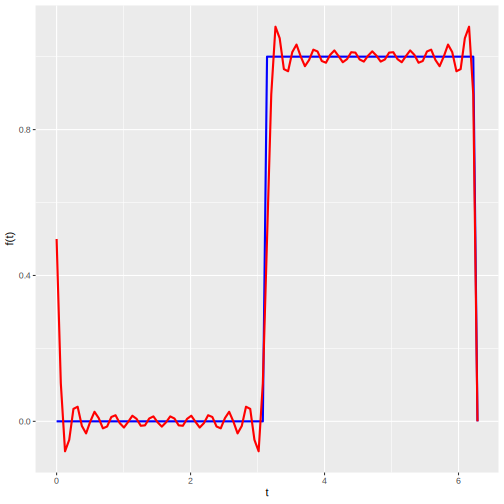
\includegraphics[width=0.7\textwidth]{media/4-1-8.pdf}
  \newline
  Aproximación de $f$ por su serie de Fourier
\end{center}

\vspace{4mm} Para $t=\pi$, tenemos que $f(\pi) = 1$, pero $s(\pi) = \frac{1}{2} - \frac{2}{\pi}\smallsum_{n=1}^\infty 0 = \frac{1}{2}$. ¿Por qué ocurre esto? ¿Cuándo se da la convergencia puntual? ¿En qué partes de la función? El siguiente apartado de esta unidad estudia estas preguntas.

\newpage
\chapter{Estudio de la convergencia puntual}
\result{Teorema de Riesz-Fisher}
\begin{onehalfspace}
  \hspace{3mm} Sea $\{\varphi_n\}_{n\in\N} \subseteq L_2(I,K)$ un sistema ortonormal. Sea $\{c_n\}_{n\in\N} \subseteq K$ que verifica $\sum_{n=0}^{\infty}|c_n|^2<\infty$. Entonces, existe una función $f$ de $L_2(I.K)$ que cumple simultáneamente:
\end{onehalfspace}
  \begin{align*}
    c_n = \langle f,\varphi_n\rangle \hspace{2mm} \forall n \in \N && \sum_{n=0}^{\infty}|c_n|^2 < ||f||^2
\end{align*}

\vspace{4mm} \dem \vspace{2mm} \newline \indent
Recordemos que la sucesión $(s_n)_n = (\smallsum_{k=0}^{n}c_k\varphi_k)_n$ es de Cauchy, pues dados $p,q \in \N$ con $p < q$, se cumple:
$$||s_p-s_q||^2 = \left|\left|\sum_{k=p+1}^{q}s_k\right|\right|^2 = \sum_{k=p+1}^{q}|c_k|^2 \xrightarrow{p,q\to\infty}0$$
Por hipótesis, $\smallsum_{k=0}^\infty |c_k|^2 < \infty$ luego el término general tiende a cero. Así, la suma de términos generales también tenderá a cero al considerar un índice inicial cada vez más alto.

\vspace{2mm} Al trabajar con un espacio de Hilbert, podemos asegurar que existe $f \in L_2(I,K)$ tal que $||s_n - f|| \xrightarrow{n\to\infty}0$. Sea $k \in \N$ cualquiera, veamos que $c_k = \langle f, \varphi_k\rangle$:
\begin{flalign*}
    \left|c_k - \langle f, \varphi_k\rangle\right| \overset{n\geq k}{=} \left|\langle s_n, \varphi_k\rangle - \langle f,\varphi_k\rangle\right| = \left|\langle s_n - f, \varphi_k\rangle\right|
\end{flalign*}
Aplicando ahora la Desigualdad de Cauchy Schwartz,
\begin{flalign*}
    \left|\langle s_n-f, \varphi_k\rangle\right| \leq ||s_n-f||\cdot ||\varphi_k|| = ||s_n - f|| \xrightarrow{n\to\infty}0
\end{flalign*}
Aplicando ahora el \hyperref[result:4.1.3]{Teorema de óptima aproximación},
$$ 0 \xleftarrow{n\to\infty} ||s_n - f|| = ||f||^2 - \sum_{k=0}^{\infty}|c_k|^2$$
Por tanto, tenemos que $\smallsum_{k=0}^\infty |c_k|^2 = ||f||^2$.

\vspace{6mm}
\result{Suma parcial como integral de semisumas}
\hspace{3mm} Sea $f\in L_2\big([0,2\pi],\R\big)$ extendida con periodo $2\pi$ a $\R$. Entonces, la suma parcial $n$-ésima de la serie de Fourier de $f$ satisface:
$$s_n(x) = \frac{a_0}{2} + \sum_{k=0}^{n}a_k \cos(kx) + b_k \sin(kx) = \frac{1}{\pi}\int_{0}^{\pi} \Big(f(x+t)+f(x-t)\Big)D_n(t) \,dt$$
$$ \text{Donde } \hspace{1mm}  D_n(t) = \begin{cases}
0 &\text{ si } t = 2\pi n \\
\frac{1}{2\sin\left(\frac{t}{2}\right)} \sin\Big((n+\frac{1}{2})\cdot t\Big) &\text{ en otro caso}
\end{cases}$$

\vspace{4mm} \dem
\vspace{2mm} \newline \indent Por definición de la suma parcial,
\begin{flalign*}
    s_n&(x) = \sum_{k=0}^{n}\langle f, \varphi_k\rangle \hspace{1mm} \varphi_k(x) = \sum_{k=0}^n \varphi_k(x) \cdot \int_{0}^{2\pi}f(t) \cdot \varphi_k(t) \,dt =&&\\[1ex]
    &=  \frac{1}{2\pi}\int_{0}^{2\pi}\hspace{-2mm} f(t) \,dt + \sum_{k=1}^{n}\left[\frac{\cos(kx)}{\pi} \int_{0}^{2\pi}\hspace{-2mm} \cos(kt) \cdot f(t) \,dt\right] + \sum_{k=1}^{n}\left[\frac{\sin(kx)}{\pi} \int_{0}^{2\pi}\hspace{-2mm} \sin(kt) \cdot f(t) \,dt\right] =\\[1ex]
    &= \frac{1}{\pi} \int_{0}^{2\pi}\left[ f(t) \left(\frac{1}{2} + \sum_{k=1}^{n} \cos(kx) \cos(kt) + \sin(kx) \sin(kt)\right)\right]\,dt = \hspace{1mm} \substack{\text{identidad trigonométrica}\\ \text{coseno de la suma}}\\[1ex]
    &= \frac{1}{\pi} \int_{0}^{2\pi} \left[f(t)\left(\frac{1}{2} + \sum_{k=1}^{n}\cos(kx - kt)\right)\right]\,dt
\end{flalign*}

\vspace{2mm}
Sea $k \leq n$ cualquiera, para $A = \frac{1}{2}(x-t)$ y $B = k(x-t)$, usamos la siguiente identidad trigonométrica: $\sin(A+B) - \sin(B-A) = 2\sin(A) \cos(B)$. Por tanto, tenemos:
$$\sin\left(\left(k+\frac{1}{2}\right) (x-t)\right)- \sin\left(\left(k-\frac{1}{2}\right) (x-t)\right) = 2 \sin\left(\frac{x-t}{2}\right) \cos\Big(k(x-t)\Big)$$

\vspace{1mm} \noindent
Sumamos ahora en $k$ hasta llegar a $n$. Al ser una suma telescópica,
$$\sin\left(\left(n+\frac{1}{2}\right)(x-t)\right) - \sin\left(\frac{x-t}{2}\right) = 2 \sin\left(\frac{x-t}{2}\right)\sum_{k=1}^{n}\cos(kx-kt)$$
\newpage
Despejando,
$$\sum_{k=1}^{n}\cos(kx-kt) = \frac{\sin\left(\left(n+\frac{1}{2}\right)(x-t)\right)}{2\sin\left(\frac{x-t}{2}\right)} - \frac{1}{2}$$
Continuamos ahora en la igualdad de la integral inicial:
\begin{flalign*}
    s_n(x) &= \frac{1}{2\pi} \int_{0}^{2\pi} f(t) \cdot \frac{\sin\left(\left(n+\frac{1}{2}\right)(x-t)\right)}{2\sin\left(\frac{x-t}{2}\right)} \,dt = \substack{\text{cambio de variable}\\u = x-t} && \\[1ex]
    &= -\frac{1}{2\pi} \int_{x}^{x-2\pi} f(x-u)\cdot D_n(u) \,du = \frac{1}{2\pi} \int_{0}^{2\pi}f(x-u) \cdot D_n(u) \,du = \\[1ex]
    &= \frac{1}{\pi}\left[\int_{0}^{\pi}f(x-u) \cdot D_n(u) \,du + \int_{\pi}^{2\pi}f(x-u) \cdot D_n(u) \,du\right] \overset{v = 2\pi - u}{=}\\[1ex]
    &= \frac{1}{\pi}\left[\int_{0}^{\pi}f(x-u)\cdot D_n(u) \,du + \int_{0}^{\pi}f(x+v)\cdot D_n(v) \,dv\right]
\end{flalign*}
Queda demostrada la igualdad. Expliquemos el último paso con algo más de detalle:
\begin{flalign*}
    \int_{\pi}^{2\pi}f(x-u) \cdot D_n(u) \,du = -\int_{\pi}^{0} f\big(x-(2\pi-v)\big)\cdot D_n(2\pi - v) \,dv
\end{flalign*}
Al ser tanto $f$ como $D_n$ funciones de periodo $2\pi$, su producto también lo es. Por tanto, podemos simplificar esta expresión para que coincida con la del enunciado.

\vspace{6mm}
\result{Lema de Riemann-Lebesgue}
\hspace{3mm} Sea $f \in L_1(J, \R)$ con $J$ un intervalo compacto real. Entonces, para $\beta \in \R$ cualquiera, se cumple:
$$ \lim_{\alpha \to \infty} \int_{J} f(t) \cdot \sin(\alpha t + \beta) \,dt = 0$$
\vspace{4mm} \dem
\vspace{2mm} \newline \indent
Sea $\varepsilon > 0$ cualquiera, pero fijo. Veamos primero que el resultado es cierto para funciones características sobre un intervalo compacto $[c,d] \subseteq J$.
\begin{adjustwidth}{0.07\textwidth}{}
    \begin{align*}
        f : J \longrightarrow \R && x \longmapsto f(x) = \begin{cases}
          1 &\text{ si } x \in [c,d] \\
          0 &\text{ si } x \in J \setminus [c,d]
        \end{cases}
    \end{align*}
    Entonces, para este caso,
    \begin{flalign*}
        \hspace{2mm} \lim_{\alpha \to \infty}& \int_J f(t) \sin(\alpha t + \beta) \,dt = \lim_{\alpha \to \infty}\int_{c}^{d}  \sin(\alpha t + \beta) \, dt = &&\\[1ex]
        &= \lim_{\alpha \to \infty} \left[\frac{-1}{\alpha} \cos(\alpha t + \beta)\right]_{t=c}^{t=d} = 0
    \end{flalign*}
    El límite es nulo al tratarse de un infinitésimo por una función acotada. Hemos comprobado que se cumple para este tipo de funciones.
\end{adjustwidth}

\vspace{4mm}
Aplicaremos ahora el siguiente resultado (no veremos su demostración):
\begin{adjustwidth}{0.07\textwidth}{}
  \vspace{2mm}
  Sean $f \in L_1([a,b], \R)$ cualquiera, $\varepsilon > 0$ cualquiera. Existen $g \in L_1([a,b], \R)$ y $s: [a,b] \longrightarrow \R$ combinación lineal de funciones características de intervalos compactos en $[a,b]$ tales que: \\[-4ex]
  \begin{align*}
      f = s+g && \int_a^b |g(t)| \,dt < \varepsilon
  \end{align*}
\end{adjustwidth}

\vspace{2mm} Así, para $\varepsilon_1 = \frac{\varepsilon}{2}$, sabemos que existen $g \in L_1(J,\R)$, $s : J \to \R$ combinación lineal de funciones características de intervalos compactos de $J$ tales que:
\begin{align*}
    f = s + g && \int_J |g(x)| \, dx < \varepsilon_1
\end{align*}
Como ya hemos demostrado el apartado anterior para funciones características, sabemos que para $\varepsilon_2 = \frac{\varepsilon}{2}$, existe $M \in \R$ tal que para todo $\alpha \geq M$ se cumple:
$$ \left|\int_J s(t) \cdot \sin(\alpha t + \beta) \, dt\right| < \varepsilon_2 = \frac{\varepsilon}{2}$$
De este modo, dado $\alpha \geq M$, tenemos:
\begin{flalign*}
    &\left| \int_J f(t) \cdot \sin(\alpha t + \beta)\,dt\right| \leq &&\\[1ex]
    &\leq\left|\int_J \Big(\underbracket{f(t) - s(t)}_{g(t)}\Big)\sin(\alpha t + \beta) \,dt\right| + \left|\int_J s(t) \cdot \sin(\alpha t + \beta) \,dt\right| \leq \\[1ex]
    &\leq \int_J \Big|g(t) \cdot \sin(\alpha t + \beta)\Big| \,dt + \varepsilon_2 \leq \int_{J} |g(t)| \,dt + \frac{\varepsilon}{2} < \varepsilon
\end{flalign*}

\result{Funciones de variación acotada}
\hspace{3mm} Sea $f : [a,b] \longrightarrow \R$ una función. Sea $\mathcal{P}([a,b])$ el conjunto de particiones del intervalo $[a,b]$. Consideraremos cada partición como:
$$p = \{a=x_0 < x_1 < \ldots < x_{n_p} = b\} \in \mathcal{P}([a,b])$$
Definimos la variación de $f$ en $[a,b]$ como:
$$V_f(a,b) = \sup_{p \in \mathcal{P}([a,b])} \sum_{i=1}^{n_p}|f(x_i) - f(x_{i-1})|$$

Si $V_f(a,b) < \infty$, se dice que ``$f$ es de variación acotada en $[a,b]$''.

\vspace{6mm}
\result{Teorema de Localización de Riemann}
\hspace{3mm} Sea $f \in L_1([0,2\pi], \R)$ una función de periodo $2\pi$ en $\R$. Entonces, la serie de Fourier de $f$ converge en $x$ si y solo si $\exists$ $\delta \in (0,\pi)$ tal que:
$$\exists \lim_{n\to\infty} \frac{2}{\pi}\int_0^\delta \frac{f(x+t)+ f(x-t)}{2} \cdot \frac{\sin\big((n+ \frac{1}{2})t\big)}{t} \,dt$$
En tal caso, converge al valor de dicho límite.

\vspace{4mm} \dem
\vspace{2mm} \newline \indent Dado $x \in \R$ cualquiera. Por el \hyperref[result:4.2.2]{resultado 4.2.2}, la serie de Fourier de $f$ converge en $x$ si y solo si:
$$\exists \lim_{n\to\infty} s_n(x) = \lim_{n\to\infty} \hspace{1mm} \frac{1}{\pi} \int_{0}^{\pi} \Big(f(x+t) + f(x-t)\Big) \cdot \frac{\sin\Big((n+\frac{1}{2})t\Big)}{2\sin(\frac{t}{2})} \,dt$$

\vspace{2mm} \noindent
Consideramos el siguiente límite auxiliar:
$$ \lim_{n\to\infty} \frac{1}{\pi} \int_{0}^{\pi} \left(\frac{1}{t} - \frac{1}{2\sin(\frac{t}{2})}\right) \cdot \Big(f(x+t) + f(x-t)\Big) \cdot \sin \left((n + \frac{1}{2})t\right)\,dt$$

\vspace{2mm}
Al ser $f \in L_1([0,2\pi], \R)$ con periodo $2\pi$ por hipótesis, $f(x-t)$ y $f(x+t)$ han de serlo también. Además, la función $\frac{1}{t} - \frac{1}{2\sin(\frac{t}{2})}$ es de variación acotada en $[0,\pi]$ (sin demostración), luego es $L_1([0,\pi], \R)$. Aplicando el \hyperref[result:4.2.3]{Lema de Riemann-Lebesgue},
\newpage
$$ \lim_{n\to\infty} \frac{1}{\pi} \int_{0}^{\pi} \left(\frac{1}{t} - \frac{1}{2\sin(\frac{t}{2})}\right) \cdot \Big(f(x+t) + f(x-t)\Big) \cdot \sin \left((n + \frac{1}{2})t\right)\,dt = 0$$
Por tanto, comparando con el límite original,
$$ \lim_{n\to\infty}s_n(x) = \lim_{n\to\infty} \frac{1}{\pi} \int_{0}^{\pi}\Big(f(x+t) + f(x-t)\Big) \cdot \frac{\sin\big((n+\frac{1}{2})t\big)}{t} \,dt$$
Sea $\delta \in (0,\pi)$ cualquiera, podemos dividir la integral como sigue:
\begin{flalign*}
    \lim_{n\to\infty} s_n(x) &= \frac{1}{\pi} \int_{0}^{\delta} \Big(f(x+t) + f(x-t)\Big) \cdot \frac{\sin\big((n+\frac{1}{2})t\big)}{t} \,dt + &\\
    &+ \frac{1}{\pi} \int_{\delta}^{\pi} \Big(f(x+t) + f(x-t)\Big) \cdot \frac{\sin\big((n+\frac{1}{2})t\big)}{t} \,dt
\end{flalign*}
El segundo sumando es nulo por el \hyperref[result:4.2.3]{Lema de Riemann-Lebesgue}.

\vspace{6mm}
\result{Teorema de Jordan}
\hspace{3mm} Si $g : [0,\delta] \longrightarrow \R$ es una función de variación acotada. Entonces, se cumple:
$$\lim_{\alpha\to\infty} \frac{2}{\pi} \int_{0}^{\delta} g(t) \cdot \frac{\sin(\alpha t)}{t}\,dt = \lim_{t \to 0^+}g(t) =: g(0^+)$$
\vspace{4mm} \dem No se verá la demostración.

\vspace{6mm}
\result{Condición de Jordan}
\hspace{3mm} Sea $f \in L_1([0,2\pi], \R)$ una función con periodo $2\pi$ que además es de variación acotada en $[x-\varepsilon, x+\varepsilon]$ para ciertos $x \in [0,2\pi]$, $\varepsilon > 0$. Entonces, la serie de Fourier de $f$ converge en $x$ si y solo si:
$$ \exists \lim_{t \to 0^+} \frac{f(x+t) + f(x-t)}{2}$$
En tal caso, converge al límite anterior.

\newpage \dem \vspace{2mm} \newline \indent
Fijado el $x$ del enunciado, tenemos que $g_1(t) := f(x-t)$ y $g_2(t) := f(x+t)$ son de variación acotada en $[-\varepsilon, \varepsilon]$. En particular, son de variación acotada en $[0,\varepsilon]$. Aplicando el \hyperref[result:4.2.6]{Teorema de Jordan},
$$ \lim_{\alpha \to \infty} \frac{2}{\pi} \int_{0}^{\varepsilon} g_1(t) \cdot \frac{\sin(\alpha t)}{t} \,dt = \lim_{t \to 0^+} g_1(t)$$
Del mismo modo,
$$ \lim_{\alpha \to \infty} \frac{2}{\pi} \int_{0}^{\varepsilon} g_2(t) \cdot \frac{\sin(\alpha t)}{t} \,dt = \lim_{t \to 0^+} g_2(t)$$
\vspace{2mm} Aplicamos ahora el \hyperref[result:4.2.5]{Teorema de Localización de Riemann} para $\delta = \varepsilon$:
\begin{flalign*}
    &\lim_{n\to\infty} \frac{2}{\pi}\int_0^\varepsilon \frac{f(x+t)+ f(x-t)}{2} \cdot \frac{\sin\big((n+ \frac{1}{2})t\big)}{t} \,dt = &&\\[1ex]
    &= \lim_{\alpha \to \infty} \frac{2}{\pi} \int_{0}^{\varepsilon}\frac{f(x+t)}{2} \cdot\frac{\sin(\alpha t)}{t} \,dt + \frac{2}{\pi} \int_{0}^{\varepsilon}\frac{f(x-t)}{2} \cdot\frac{\sin(\alpha t)}{t} \,dt =\\[1ex]
    &= \lim_{t\to 0^+} \frac{f(x+t) + f(x-t)}{2}
\end{flalign*}
Como el \hyperref[result:4.2.5]{Teorema de Localización de Riemann} garantiza la convergencia al valor del límite, concluimos la demostración.

\vspace{6mm}
\result{Teorema de Dini}
\hspace{3mm} Sea $g : [0,b] \longrightarrow \R$ tal que $\exists \lim_{t\to 0^+}g(t) =: g(0^+)$. Entonces, si existe $\delta \in (0,b)$ tal que
$$ \frac{g(t) - g(0^+)}{t} \in L_1([0,\delta], \R)$$

\vspace{2mm} \noindent se verifica: \vspace{2mm}
$$ \lim_{\alpha \to \infty} \frac{2}{\pi} \int_{0}^{\delta} g(t) \cdot \frac{\sin(\alpha t)}{t} \,dt = g(0^+)$$

\newpage \dem \vspace{2mm} \newline \indent
Supongamos que existe tal $\delta \in (0, b)$. Así, podemos reescribir el límite del enunciado como:
\begin{flalign*}
    &\lim_{\alpha \to \infty} \frac{2}{\pi} \int_{0}^{\delta} g(t) \cdot \frac{\sin(\alpha t)}{t} \,dt =\\[1ex]
    &= \lim_{\alpha \to \infty} \frac{2}{\pi} \int_{0}^{\delta} \Big(g(t) - g(0^+)\Big) \cdot \frac{\sin(\alpha t)}{t} \,dt + \frac{2}{\pi} \int_{0}^{\delta} g(0^+) \cdot \frac{\sin(\alpha t)}{t} \,dt
\end{flalign*}
\vspace{2mm}
Por hipótesis, $\frac{g(t) - g(0^+)}{t} \in L_1([0,\delta], \R)$. Aplicando el \hyperref[result:4.2.3]{Lema de Riemann-Lebesgue},
$$\lim_{\alpha \to \infty} \frac{2}{\pi} \int_{0}^{\delta} \frac{g(t) - g(0^+)}{t} \cdot \sin(\alpha t)\,dt = 0$$
\vspace{2mm} Volviendo a la igualdad anterior,
\begin{flalign*}
  \hspace{3ex} &\lim_{\alpha \to \infty} \frac{2}{\pi} \int_{0}^{\delta} g(t) \cdot \frac{\sin(\alpha t)}{t} \,dt = \lim_{\alpha \to \infty}  \frac{2}{\pi} \int_{0}^{\delta} g(0^+) \cdot \frac{\sin(\alpha t)}{t} \,dt =&&\\[1ex]
  &= \frac{2}{\pi}\cdot g(0^+) \lim_{\alpha \to \infty} \int_{0}^{\delta} \frac{\sin(\alpha t)}{t} \,dt \overset{u = \alpha t}{=} \frac{2}{\pi}\cdot g(0^+) \int_{0}^{\infty} \frac{\sin(u)}{u}\,du = g(0^+)
\end{flalign*}
El último paso se debe a ser la integral bien conocida.

\vspace{6mm}
\result{Condición de Dini}
\begin{onehalfspace}
  \hspace{3mm} Sea $f \in L_1([0,2\pi], \R)$ con periodo $2\pi$. Fijado $x \in \R$ cualquiera, consideramos la función $g(t) := \frac{f(x+t) + f(x-t)}{2}$. Si existen $g(0^+) := \mlim{t\to0^+}$ y $\delta > 0$ tal que la función $\frac{g(t) - g(0^+)}{t}\in L_1([0,\delta], \R)$. Entonces, la serie de Fourier de $f$ converge en $x$ y lo hace al valor:
\end{onehalfspace}
  $$\lim_{t \to 0^+} \frac{f(x+t)+f(x-t)}{2}$$

\vspace{4mm} \dem Análoga a \hyperref[result:4.2.7]{la condición de Jordan}.
\newpage \indent Al ser $f$ $2\pi$-periódica por hipótesis, también ha de serlo $g$. Razonando como en la Condición de Jordan,
\begin{flalign*}
    &\lim_{n\to\infty} \frac{2}{\pi}\int_0^\delta \frac{f(x+t)+ f(x-t)}{2} \cdot \frac{\sin\big((n+ \frac{1}{2})t\big)}{t} \,dt = &&\\[1ex]
    &= \lim_{\alpha \to \infty} \frac{2}{\pi} \int_{0}^{\delta}\frac{f(x+t)}{2} \cdot\frac{\sin(\alpha t)}{t} \,dt + \frac{2}{\pi} \int_{0}^{\delta}\frac{f(x-t)}{2} \cdot\frac{\sin(\alpha t)}{t} \,dt =\\[1ex]
    &= \lim_{t\to 0^+} \frac{f(x+t) + f(x-t)}{2}
\end{flalign*}
Hemos aplicado el \hyperref[result:4.2.6]{Teorema de Dini} al primer sumando (las hipótesis de este enunciado nos garantizan las condiciones para ello), y el \hyperref[result:4.2.3]{Lema de Riemann-Lebesgue} al segundo.

\vspace{6mm}
\result{Teorema de Carleson}
\hspace{3mm} Si $f \in L_2([0,2\pi],\R)$; entonces, la serie de Fourier de $f$ converge y además converge a $f(x)$ en casi todo punto.

\vspace{2mm} \dem Sin demostración.

\vspace{2mm}
La continuidad no basta para garantizar la convergencia puntual. ¿Que propiedades sí nos puede garantizar la continuidad?

\vspace{6mm}
\result{Ejemplo sobre una función concreta}
\hspace{3mm} Consideramos la función $f(x) = x$ en $[0,2\pi]$ extendida periódicamente a $\R$. Veamos cómo calcular su serie de Fourier y estudiemos su convergencia puntual.
$$f(x) \sim \frac{a_0}{2} + \sum_{n=1}^{\infty}\Big[a_n \cos(nx) + b_n \sin(nx)\Big]$$
Comencemos calculando los coeficientes:
\begin{flalign*}
    a_0 = \frac{1}{\pi} \int_0^{2p\pi} f(t) \,dt = \frac{1}{\pi} \int_0^{2\pi}t\,dt = \frac{1}{\pi} \cdot \frac{2^2 \pi^2}{2} = 2\pi&&
\end{flalign*}
\newpage
\begin{flalign*}
    a_n &= \frac{1}{\pi}\int_0^{2\pi} f(t) \cdot \cos(nt) \,dt = \frac{1}{\pi}\left[\frac{t \sin(nt)}{n} - \frac{1}{n} \int \sin(nu) \,du\right]_{t=0}^{t=2\pi} =&&\\[1ex]
    &= \frac{1}{\pi} \left[\frac{t \sin(nt)}{n} + \frac{\cos(nt)}{n^2}\right]_{t=0}^{t=2\pi} = \frac{1}{\pi} \left(\frac{\cos(2n\pi)}{n^2} - \frac{\cos(0)}{n^2}\right) = 0
\end{flalign*}
\begin{flalign*}
    b_n &= \frac{1}{\pi}\int_0^{2\pi} f(t) \cdot \sin(nt) \,dt = \frac{1}{\pi}\left[\frac{-t \cos(nt)}{n} - \frac{1}{n} \int -\cos(nu) \,du\right]_{t=0}^{t=2\pi} =&&\\[1ex]
    &= \frac{1}{\pi} \left[\frac{-t \cos(nt)}{n} + \frac{\sin(nt)}{n^2}\right]_{t=0}^{t=2\pi} = \frac{1}{\pi} \left(\frac{0\cdot\cos(0)}{n} - \frac{2\pi \cos(2n\pi)}{n}\right) = -\frac{2}{n}
\end{flalign*}
De este modo,
$$ f(x) \sim \pi - 2\sum_{n=1}^{\infty}\frac{\sin(nx)}{n}$$

\vspace{4ex}
\begin{minipage}{0.5\textwidth}
  \begin{center}
  \includegraphics[width=0.7\textwidth]{media/4-2-11a.pdf}
  \newline
  Representación de $f$
\end{center}
\end{minipage}
\begin{minipage}{0.5\textwidth}
  \begin{center}
  \includegraphics[width=0.7\textwidth]{media/4-2-11b.pdf}
  \newline
  Serie de Fourier de $f$ con 20 términos
\end{center}
\end{minipage}

$\bullet$ Condición de Jordan: Si $x \in [0,2\pi)$, $f$ es monótona y por tanto este variación acotada en $(x-\delta, x+\delta)$ para cierto $\delta > 0$. Si $x = 0$ ó $x = 2\pi$, $f$ es suma de funciones monótonas luego también es de variación acotada en $(x-\delta, x+\delta)$ para cierto $\delta > 0$. De este modo, la serie de Fourier de $f$ converge $\forall \hspace{1mm} x \in \R$, y lo hace al valor:
$$\lim_{t\to 0^+} \frac{f(x+t)+f(x-t)}{2}$$
\indent Tenemos que para todo $x\in (0,2\pi)$ converge a $f(x) = x$, y para $x \in \{0,2\pi\}$ converge a $\frac{0+2\pi}{2} = \pi$. Estas convergencias pueden extenderse por periodicidad en $\R$.

\vspace{4mm}
Por tanto, $\forall \hspace{1mm} x \in (0,2\pi)$ se cumple:
$$x = \pi - 2\sum_{n=1}^{\infty}\frac{\sin(nx)}{n} \overset{x = \frac{\pi}{2}}{\Rightarrow} \frac{\pi}{4} = \sum_{n=1}^{\infty}\frac{(-1)^n}{2n+1}$$

$\bullet$ Condición de Dini: Para $x \in [0,2\pi]$ fijo, consideramos la siguiente función auxiliar con periodo $2\pi$: 
\vspace{2mm}
$$g(t) := \frac{f(x+t) + f(x-t)}{2}$$ \vspace{2mm}
\begin{onehalfspace}
Para el caso $x\in (0,2\pi)$, tenemos que $g(t) = \frac{t-t}{2} = 0$. Además, existe $g(0^+) = 0$ y se cumple:
$$ \frac{g(t) - g(0^+)}{t} = \frac{0}{t} = 0 \in L_1([0,\delta], \R)\text{ para cierto } \delta > 0$$
Por tanto, la serie de Fourier de $f$ converge a $g(0^+) = x$ para cualquier $x \in (0,2\pi)$.
\end{onehalfspace}

\vspace{4mm}
Si $x \in \{0,2\pi\}$, $g(t) =  \frac{2\pi+t-t}{2} = \pi$ luego $g(0^+) = \pi$. De este modo,
$$ \frac{g(t) - g(0^+)}{t} = \frac{\pi - \pi}{t} = 0 \in L_1([0,\delta], \R)\text{ para cierto } \delta > 0$$
En este caso, la serie de Fourier de $f$ converge a $g(0^+) = \pi$.

\vspace{4mm}
\nota La continuidad no basta para garantizar la convergencia puntual.

\vspace{6mm}
\result{Definición de convergencia Cesàro}
\hspace{3mm} Sea $(a_n)_{n\in\N}$ una sucesión de números reales. Sea $(s_n)_{n\in\N} = (\smallsum_{k=1}^n a_k)_{n\in\N}$ la correspondiente sucesión de sumas parciales. Se dice que $\smallsum_{n=1}^\infty a_n$ es sumable Cesàro si verifica:
$$\exists \lim_{n\to\infty} \sigma_n = \lim_{n\to\infty} \frac{1}{n} \sum_{k=1}^{n} s_k = \sigma \in \R$$
En tal caso, diremos que $\sigma$ es la ``suma Cesàro de la serie''.

\vspace{6mm}
\nota Sin demostración:
\vspace{2mm} \newline \indent Si $\smallsum_{n=1}^{\infty}a_n$ converge a $s$; entonces, $a_n$ es sumable Cesàro a $\sigma = s$.

\newpage
\result{Teorema de Fejèr}
\hspace{3mm} Dada una función $f \in L_1([0,2\pi],\R)$ con periodo $2\pi$ en $\R$. Consideramos la siguiente función:
$$s(x) := \lim_{t\to 0^+} \frac{f(x+t)+f(x-t)}{2} \hspace{3mm} \text{ en } x \in A := \Big\{x \in [0,2\pi] : s(x) \text{ bien definida}\Big\}$$
Entonces, la serie de Fourier de $f$ converge Cesàro $\forall \hspace{1mm} x \in A$ a $s(x)$.

\vspace{4mm}
Además, si $f$ es continua en $\R$, las sumas de Fejèr ($\sigma_n$) convergen de manera uniforme a $s$ en $A = \R$; es decir,
$$\forall \hspace{1mm} \varepsilon > 0 \hspace{2mm} \exists \hspace{1mm} n_0 \in \N : |\sigma_n(x) - s(x)| < \varepsilon \hspace{2mm}  \forall x \in \R \hspace{2mm} \forall n \geq n_0$$

\vspace{4mm} \dem Sin demostración.

\vspace{6mm}
\result{Propiedades de funciones continuas}
\hspace{3mm} Sea $f$ una función continua en $\R$ con periodo $2\pi$; entonces,
\begin{enumerate}[label=\roman*)]
    \item $||s_n - f|| \xrightarrow{n\to\infty}0$
    \item Se cumple la identidad de Parseval en $[0,2\pi]$:
    $$ ||f||^2 = \sum_{k=0}^{\infty} |c_k|^2 = \frac{a_0^2}{4} + \sum_{n=1}^{\infty} a_n^2 + b_n^2$$
    \item Si la serie de Fourier de $f$ converge en $x$, converge a $f(x)$.
    \item La serie de Fourier es integrable término a término:
    $$\int_0^x f(t) \,dt = \frac{a_0}{x} + \sum_{n=1}^{\infty} \int_0^x a_n \cos(nt) + b_n \sin(nt) \,dt$$
\end{enumerate}
\vspace{4mm}
\dem
\vspace{2mm} \newline \indent
\begin{tcolorbox}[Subset-contingency]
  $\romannumeral 1$ \hspace{3mm} Al ser $f$ continua, es $L_2([0,2\pi], \R)$. Basta aplicar el \hyperref[result:4.2.10]{Teorema de Carleson}.
\end{tcolorbox}
\vspace{2mm}
\begin{tcolorbox}[Subset-contingency]
  $\romannumeral 2$ \hspace{3mm} Se tiene al haber usado un \hyperref[result:4.1.8]{sistema ortonormal completo}.
\end{tcolorbox}

\end{document}